% This project is a template slides for the subsequent presentations which are significant during the postgraduate period.
% Template for College of Information Science and Electronic Engineering, Zhejiang University.
% Compiled with pdflatex.
% By Xue Shengke.

\documentclass[10pt, mathserif]{beamer}	% font and size
\mode<presentation>
{
	\setbeamercovered{dynamic}	% translucent when using pause
	\setbeamertemplate{navigation symbols}{}	% hide navigation bars
	\setbeamertemplate{caption}[numbered]	% numerate captions
	\setbeamertemplate{background}{
\includegraphics[height=\paperheight]{ISEE.pdf}}	% set background image
	\setbeamertemplate{footline}{\textcolor{light-gray}{\scriptsize \insertframenumber/\inserttotalframenumber} \hfill}	% display page number at bottom left corner	
}
%\usepackage{ctex}
\usepackage{xeCJK}
\usepackage{times}		% font for english, Times New Roman
\usepackage{amsmath, amsfonts, amssymb}	% math equations, symbols
\usepackage[english]{babel}
\usepackage{color}		% color content
\usepackage{graphicx}	% import figures
\usepackage{subfigure}
\usepackage{url}		% hyperlinks
\usepackage{bm}			% bold type for equations
\usepackage{hyperref}	% bookmarks
\hypersetup{bookmarks, unicode}	% unicode
\setCJKfamilyfont{hei}{SimHei}                                    %黑体  hei
\newcommand{\hei}{\CJKfamily{hei}}   	% all Chinese should be enclosed between the commands
\newcommand{\xiaowu}{\fontsize{9pt}{\baselineskip}\selectfont}
\usepackage{setspace}
\renewcommand{\baselinestretch}{1.3}
\newcommand{\ftitle}[1]{\frametitle{#1}}	% userdefine frametitle
\definecolor{light-gray}{gray}{0.90}

\providecommand{\tightlist}{%

  \setlength{\itemsep}{0pt}

  \setlength{\parskip}{0pt}

  \setlength{\itemindent}{1em}

}

\hypersetup{hidelinks}

\def\equationautorefname        {式}
\def\footnoteautorefname        {脚注}
\def\figureautorefname          {图}
\def\tableautorefname           {表}
\def\partautorefname            {篇}
\def\chapterautorefname         {章}
\def\sectionautorefname         {节}
\def\subsectionautorefname      {小节}
\def\subsubsectionautorefname   {小小节}
\def\paragraphautorefname       {段落}
\def\subparagraphautorefname    {子段落}
\def\appendixautorefname        {附录}
\def\FancyVerbLineautorefname   {行}
\def\theoremautorefname         {定理}
\def\listoffigures              {代码}
\def\lstlistingname             {代码}

\begin{document}

\title[abbreviation]{高速低功耗流水线ADC子电路设计(2.0)}
\author{ 何扬槊 \\ 3180102687@zju.edu.cn}
\institute[ISEE]{\normalsize 
		
\includegraphics[width=0.2\textwidth]{ZJU_BLUE.pdf}  \\  % add a special logo on cover page
	College of Information Science and Electronic Engineering \\
	信息与电子工程学院 \\
	浙江大学
	}
\date{Winter, 2019}

\AtBeginSection[]
{
\begin{frame}
   	\ftitle{Outline 目录}		% contents for better review
    \tableofcontents[currentsection, currentsubsection]
\end{frame}
}

\begin{frame}
    \titlepage	% make the cover page here
\end{frame}

\section{First 高速低功耗ADC的需求}
\begin{frame}
	\ftitle{高速低功耗ADC的需求}
	5G时代的到来,对ADC转换器提出了更高的要求。
	\begin{figure}[ht]
        \centering
        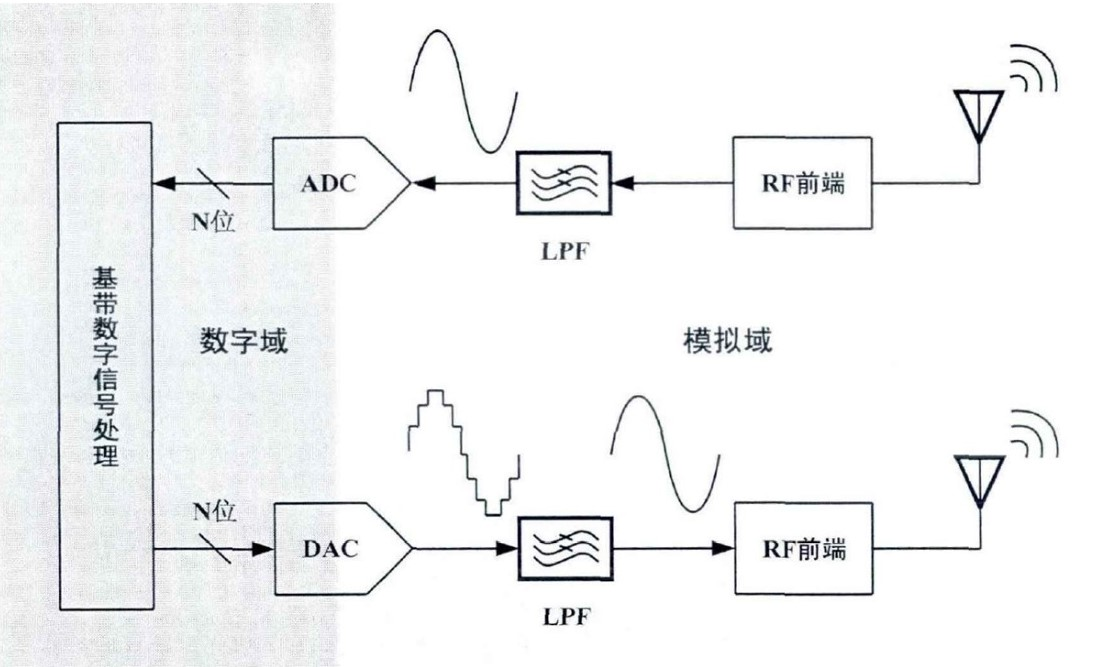
\includegraphics[width=8cm]{ADCDAC.jpg}
        \caption{\label{fig:ADCDAC}几款国外商用ADC芯片指标}
    \end{figure}
\end{frame}

\begin{frame}
	\ftitle{高速低功耗ADC的需求}
	一方面,基站密度上升,手机使用量增加,收发毫米波等级的信号,使得芯片的功耗增长巨大。
	\par 另一方面,随着高频频段的引入,超高速、高精度是5G时代ADC不可或缺的特征。
	\\ \hspace*{\fill} \\
	\par Pipeline ADC是一种折中的考虑,能够用较少比较器得到较高精度,
    往往是高速、高精度ADC的首选。
\end{frame}

\section{Second SHA-less架构系统级仿真}

	\begin{frame}
		\ftitle{热噪声模型}
		\par 对功率谱积分得到其总噪声功率:
		\begin{equation}
			\begin{split}
				P_{n\_\text {tolal}} = \frac{kT}{C_s}
			\end{split}
		\end{equation}
		\par 如\autoref{fig:kTnoise},利用随机波形与总噪声幅度
		相乘,得到其噪声模型。
		\begin{figure}[H]
			\centering
			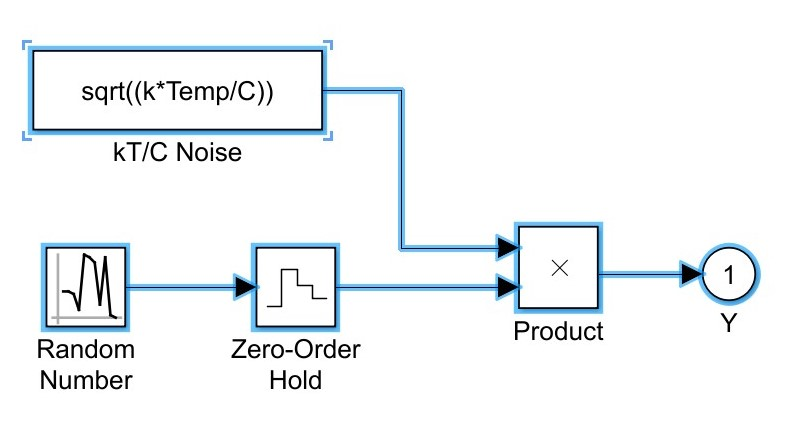
\includegraphics[width=7cm]{kTnoise}
			\caption{\label{fig:kTnoise}开关热噪声行为级仿真}
		\end{figure}
	\end{frame}

	\begin{frame}
		\ftitle{热噪声模型}
		\par 运放的热噪声主要是MOS管的沟道噪声,根据MOS管小信号等效模型,可以推导出运放噪声功率:
		\begin{align}
		P_{n,opa} \propto \frac{kT}{C_T}
		\end{align}
		\par 如\autoref{fig:Opnoise},利用随机波形与总噪声幅度
		相乘,得到模型。
		\begin{figure}[H]
			\centering
			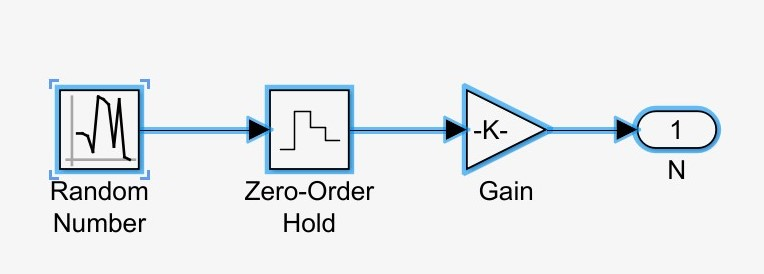
\includegraphics[width=8cm]{Opnoise}
			\caption{\label{fig:Opnoise}运放热噪声行为级仿真}
		\end{figure}
	\end{frame}

	\begin{frame}
		\ftitle{热噪声模型}
		在实际的S/H电路中,还有时钟抖动引起的噪声,设输入信号为$ f(t) $
		\begin{align}
			V_{in}(t) & = V_{in,ideal}(t) + \frac{dV_{in}(t)}{dt}\Delta t 
		\end{align}

		如\autoref{fig:jitter}所示,
		利用随机数生成器与输入信号瞬时斜率相乘,再进行输出。
		\begin{figure}[H]
			\centering
			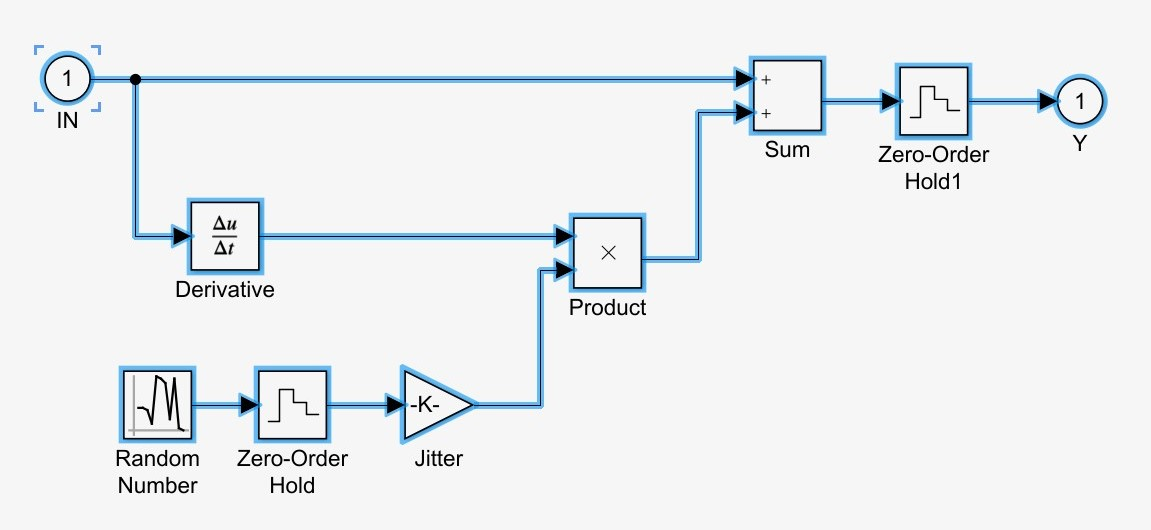
\includegraphics[width=8cm]{jitter}
			\caption{\label{fig:jitter}时钟抖动噪声行为级模型}
		\end{figure}
	\end{frame}

	\begin{frame}
		\ftitle{热噪声模型}
		\par 同时,S/H电路中的运算放大器工作在闭环模式,由于实际运放增益$ A_v \neq \infty $,
		则运放的闭环增益将会存在一定非线性误差
		\begin{align}
			V_{out} = V_{in}\frac{A_v}{1+\beta A_v}
		\end{align}
		\par 如\autoref{fig:gainerror}所示,利用函数模块Fcn可以大致实现运放增益误差模型,
		\begin{figure}[H]
			\centering
			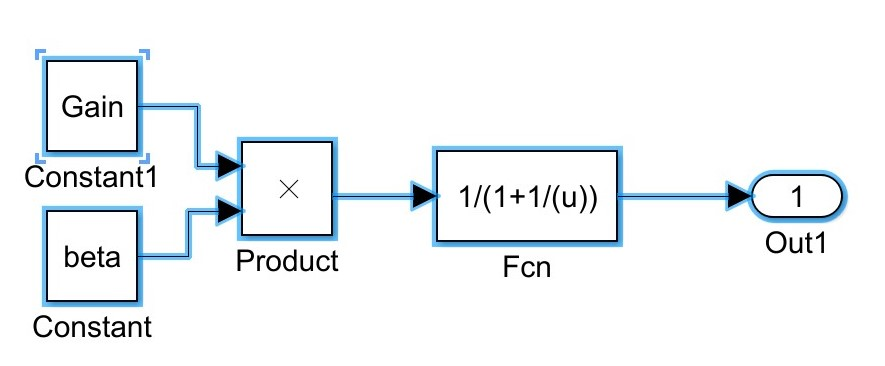
\includegraphics[width=7cm]{gainerror}
			\caption{\label{fig:gainerror}运放闭环增益误差行为级模型}
		\end{figure}
	
	\end{frame}


	\begin{frame}
		\ftitle{非理想状态下12bit流水线ADC仿真}
		根据上述对S/H电路非理想性的分析,整合出同时考虑多种非理想因素的
		S/H电路simulink模型,如\autoref{fig:SH_sim1}所示。
		\begin{figure}[H]
			\centering
			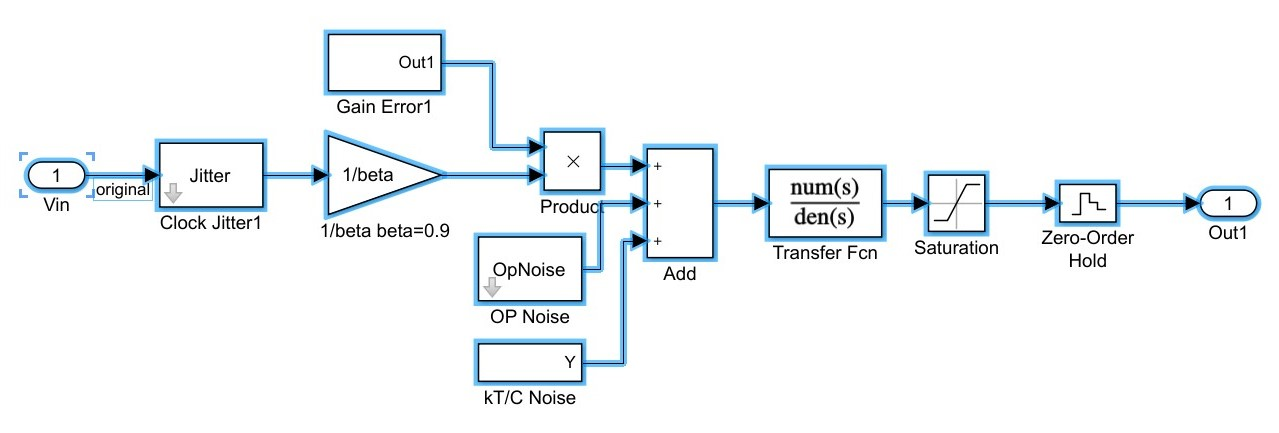
\includegraphics[width=10cm]{SH_sim1}
			\caption{\label{fig:SH_sim1}考虑非理想因素的S/H电路行为级模型}
		\end{figure}		
	\end{frame}

	\begin{frame}
		\ftitle{非理想状态下12bit流水线ADC仿真}
		仿真结果如7(a)和7(b)所示,
    	在考虑诸多非理想性后性能有了明显的下降,信噪失真比SNDR仅9.92dB,有效位数ENOB仅1.36
		\begin{figure}[H]
			\centering
			\subfigure[传统流水线ADC输出]{
			\begin{minipage}[t]{0.5\linewidth}
			\centering
			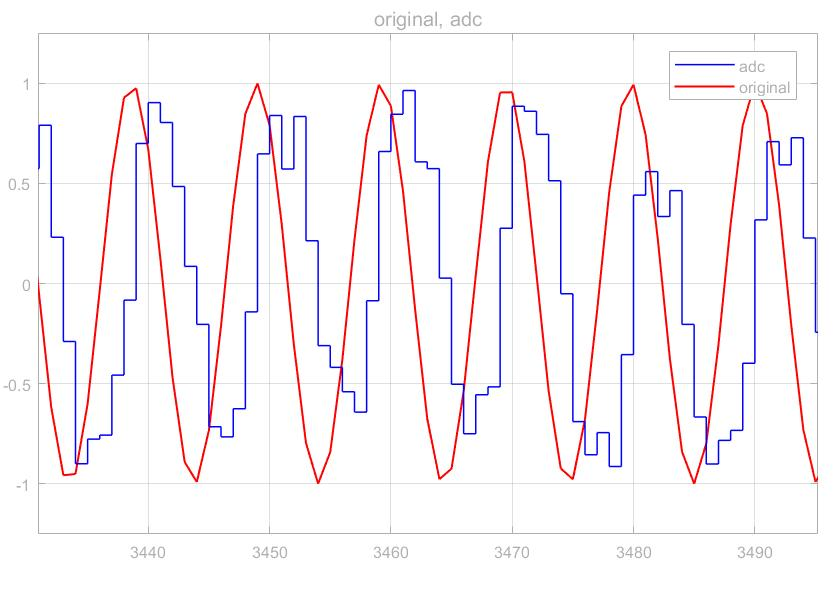
\includegraphics[width=5cm]{ADC_out1}
			\end{minipage}%
			}%
			\subfigure[传统流水线ADC频谱]{
			\begin{minipage}[t]{0.5\linewidth}
			\centering
			\includegraphics[width=5cm]{ADC_spectrum1}
			\end{minipage}%
			}%
			\centering
			\caption{仿真结果}
		\end{figure}

	\end{frame}

	\begin{frame}
		\ftitle{非理想状态下12bitSHA-less流水线ADC仿真}
		由于第一级子结构的
    	输入信号变为了直接输入,导致了MDAC与sub-ADC处理的信号存在不一致现象,
    	也被称作孔径误差。
		\par 将最前端的S/H电路去除,重新进行仿真结果如7(a)和7(b)所示。
		\begin{figure}[H]
			\centering
			\subfigure[传统流水线ADC输出]{
			\begin{minipage}[t]{0.5\linewidth}
			\centering
			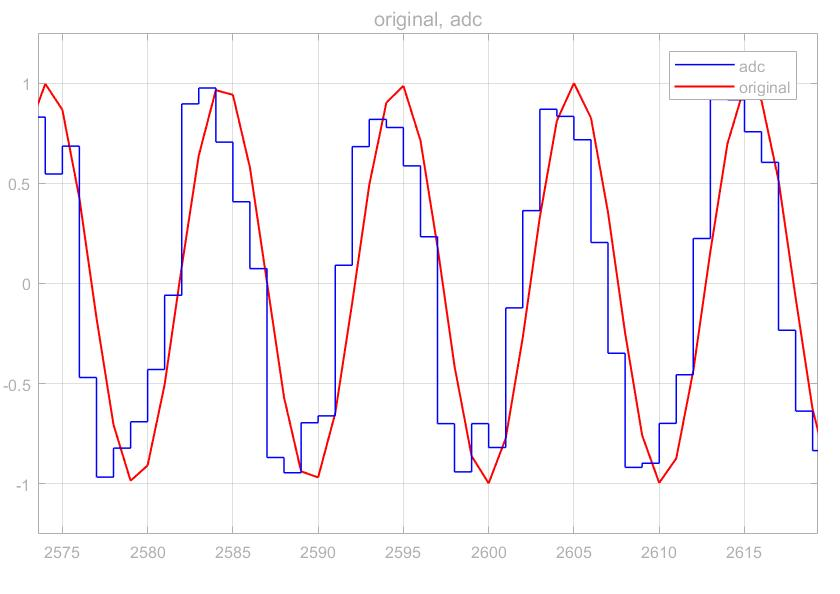
\includegraphics[width=5cm]{ADC_out2}
			\end{minipage}%
			}%
			\subfigure[传统流水线ADC频谱]{
			\begin{minipage}[t]{0.5\linewidth}
			\centering
			\includegraphics[width=5cm]{ADC_spectrum2}
			\end{minipage}%
			}%
			\centering
			\caption{仿真结果}
		\end{figure}

	\end{frame}

\section{Third 子电路设计}

	\begin{frame}
		\ftitle{运算放大器}
		\begin{table}[H]
			\centering
			\begin{tabular}{|c|c|c|}
			\hline
			Parameters & Requirements & Result \\ \hline
			static power & $ \leq 2mW  $ & $ 0.81mW $ \\ \hline
			open loop gain & $ 73.98dB $ & $ 80.29dB $ \\ \hline
			GBW & $ 5MHz $ & $ 5.012MHz $ \\ \hline
			$\phi$ & $ \geq 60^\circ $ & $ 67.3^\circ $ \\ \hline
			SR & $ \geq 10V/\mu s $ & $ 7.43,\ 10.72(V/\mu s) $ \\ \hline
			CMRR & none & $ 84.82dB $ \\ \hline
			output voltage swing & $ [-2V,\ 2V] $ & $ [-2.2292V,\ 2.186V] $ \\ \hline
			ICMR & $ [-2V,\ 1V] $ & $ [-2.369V,\ 1.23V] $ \\ \hline
			\end{tabular}
			\caption{\label{tab:all}电路总体参数}	

				
		\end{table} 
	\end{frame}

	\begin{frame}
		\ftitle{栅压自举式开关}
		电路如\autoref{fig:boot}所示。
		当处于“关”状态时,MN1导通,$ C_b $下极板接地。
		节点n4为低电平,则MP2导通,此时$ C_b $上极板接VDD。
		MN7断开,MP4导通,MP1断开,从而将MS与$ C_b $断开.
		\par 当处于“开”状态时,MN4导通MP1的G极接低电压,而S
		极接高电压,MP1导通。节点n4为高电平,所以MN7和MS导通。
		\begin{figure}[ht]
			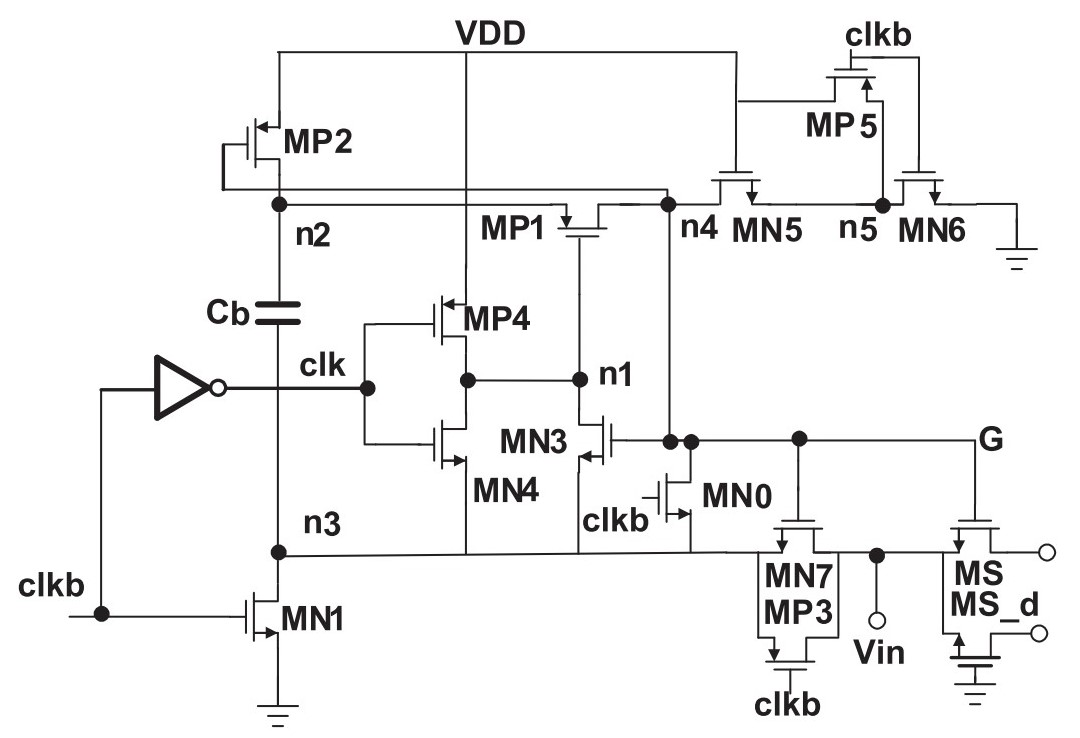
\includegraphics[width=5cm]{boot}
			\caption{\label{fig:boot}栅压自举式开关电路}
		\end{figure}		
	\end{frame}

	\begin{frame}
		\ftitle{栅压自举式开关}
		\par \autoref{fig:bootstrap_d}为输出结果,
		同时利用MATLAB画图功能对其压摆率进行测试
		\begin{align}
			SR = \frac{1.152V-0.1372V}{0.0002\mu s} = 5074V/\mu s
		\end{align}
		\begin{figure}[H]
			\centering
			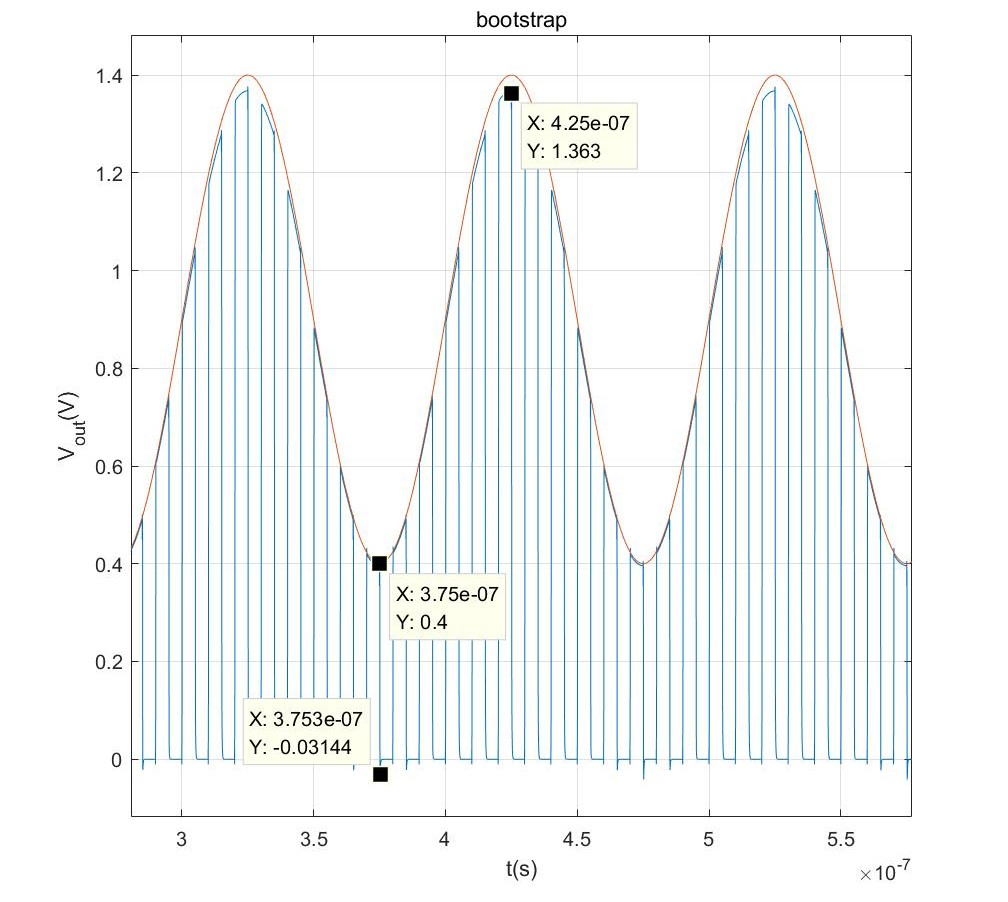
\includegraphics[width=5cm]{bootstrap_d}
			\caption{\label{fig:bootstrap_d}栅压自举式开关输出信号}
		\end{figure}
	\end{frame}

	\begin{frame}
		\ftitle{S/H电路}
		\par 从电路简易性与电路功耗的角度来说如\autoref{fig:switch}的采样电路较为合适。
		\begin{figure}[H]
			\centering
			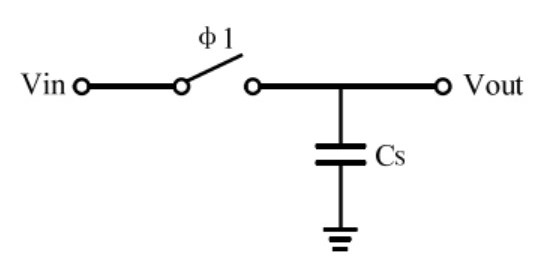
\includegraphics[width=5cm]{switch}
			\caption{\label{fig:switch}简单的采样开关电路}
		\end{figure}		
	\end{frame}

	\begin{frame}
		\ftitle{S/H电路}
		\par 利用HSPICE仿真,可以得到该S/H电路的输出。令输入
		信号为正弦波,输出信号如\autoref{fig:SH_simple}。对该电路的功耗进行仿真可得
		\begin{align}
			P_{SH} = 72.46\mu W
		\end{align}	
		\begin{figure}[H]
			\centering
			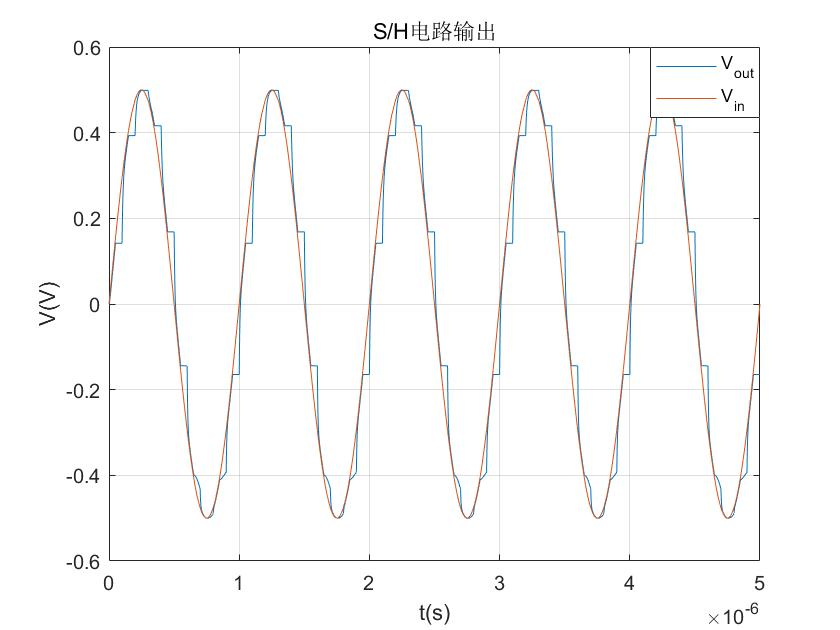
\includegraphics[width=5cm]{SH_simple}
			\caption{\label{fig:SH_simple}简单的S/H电路输出}
		\end{figure}

	\end{frame}

	\begin{frame}
		\ftitle{动态比较器}
		\par 当clk为低电平时,比较器在复位阶段,M1和M2的D极,节点ON与OP经M5与M6两侧的PMOS管接到VDD。
		当clk为高电平时,M7导通,节点DN与DP电压下降,由于M1与M2的G极电压不同($ V_{ip} < V_{in} $),
		若DP更快,当$ V_{DP} < VDD - V_{TN} $时,M6导通,M4导通,从而节点OP电压
		下降,节点ON电压上升,经过反相器后,输出高电平。
		\begin{figure}[H]
			\centering
			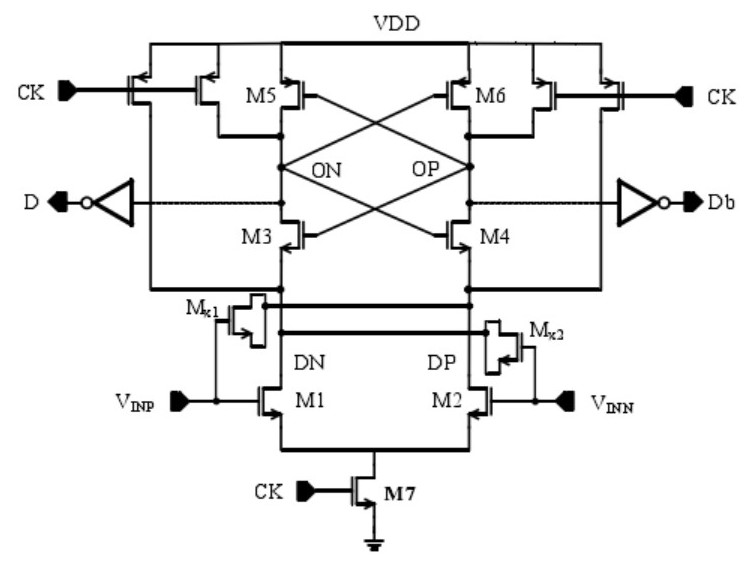
\includegraphics[width=5cm]{comparator}
			\caption{\label{fig:comparator}动态比较器电路}
		\end{figure}
	\end{frame}

	\begin{frame}
		\ftitle{动态比较器}
		\par 利用HSPICE仿真,可以得到动态比较器的大致性能,如\autoref{fig:comparator_perform}。
		\begin{figure}[H]
			\centering
			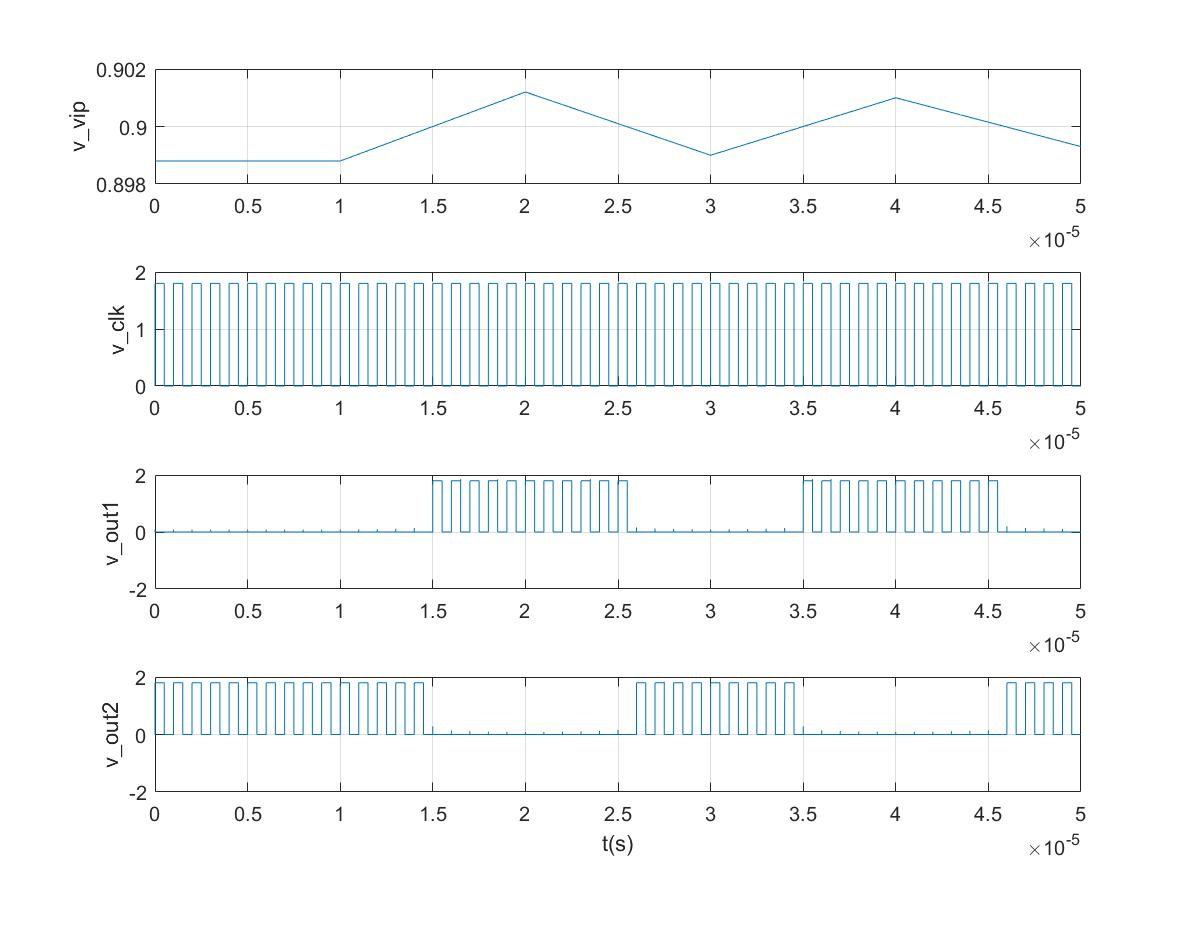
\includegraphics[width=7cm]{comparator_perform}
			\caption{\label{fig:comparator_perform}动态比较器仿真}
		\end{figure}
	\end{frame}

	\begin{frame}
		\ftitle{动态比较器}
		\par 经过查询HPSICE仿真得到的.lis文件
		可以大致计算压摆率
		\begin{align}
			SR = \frac{1.6043V-0.1526V}{5.0002645\mu s-5.000236\mu s} = 5.09\times10^{4}V/\mu s
		\end{align}
		\begin{figure}[H]
			\centering
			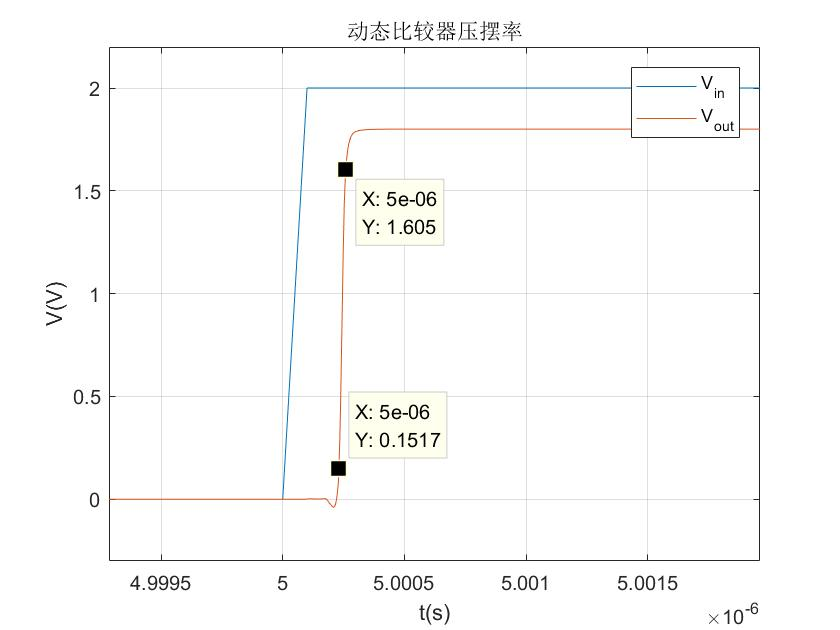
\includegraphics[width=6cm]{comparator_SR}
			\caption{\label{fig:comparator_SR}动态比较器压摆率}
		\end{figure}
	\end{frame}

	\begin{frame}
		\ftitle{sub-ADC电路}
		sub-ADC采用全平行结构ADC,论文采用的第一级子结构为2.5bitMDAC,因此对应的sub-ADC需要6个比较器
		对应的参考电压为:
		\begin{align*}
			V_{ref1} & = -0.625,\ V_{ref2} = -0.375 \\
			V_{ref3} & = -0.125, \ V_{ref4} = 0.125 \\
			V_{ref5} & = 0.375,\ V_{ref6} = 0.625 
		\end{align*}
		由于论文仅涉及流水线ADC的子结构部分,
    	而未对后续的数字校正电路实现,因此,此处sub-ADC的输出仅为6个比较器的输出,而非对应的数字码。
	\end{frame}

	\begin{frame}
		\ftitle{sub-ADC电路}
		\par sub-ADC电路原理图如\autoref{fig:subADC_multisim}。
		\begin{figure}[H]
			\centering
			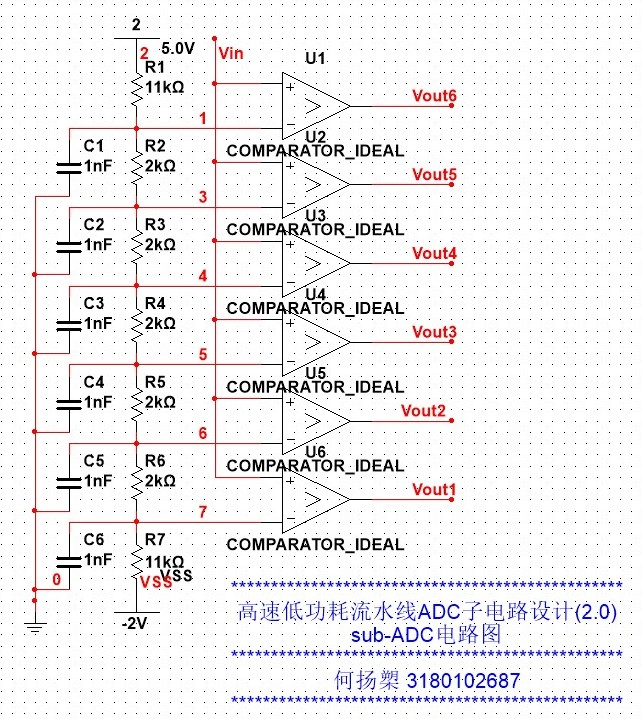
\includegraphics[width=5.5cm]{subADC_multisim}
			\caption{\label{fig:subADC_multisim}sub-ADC电路原理图}
		\end{figure}		
	\end{frame}

	\begin{frame}
		\ftitle{sub-ADC电路}
		\par 利用HSPICE仿真,可以得到sub-ADC的输出波形,如\autoref{fig:subADC_out}。
		\begin{figure}[H]
			\centering
			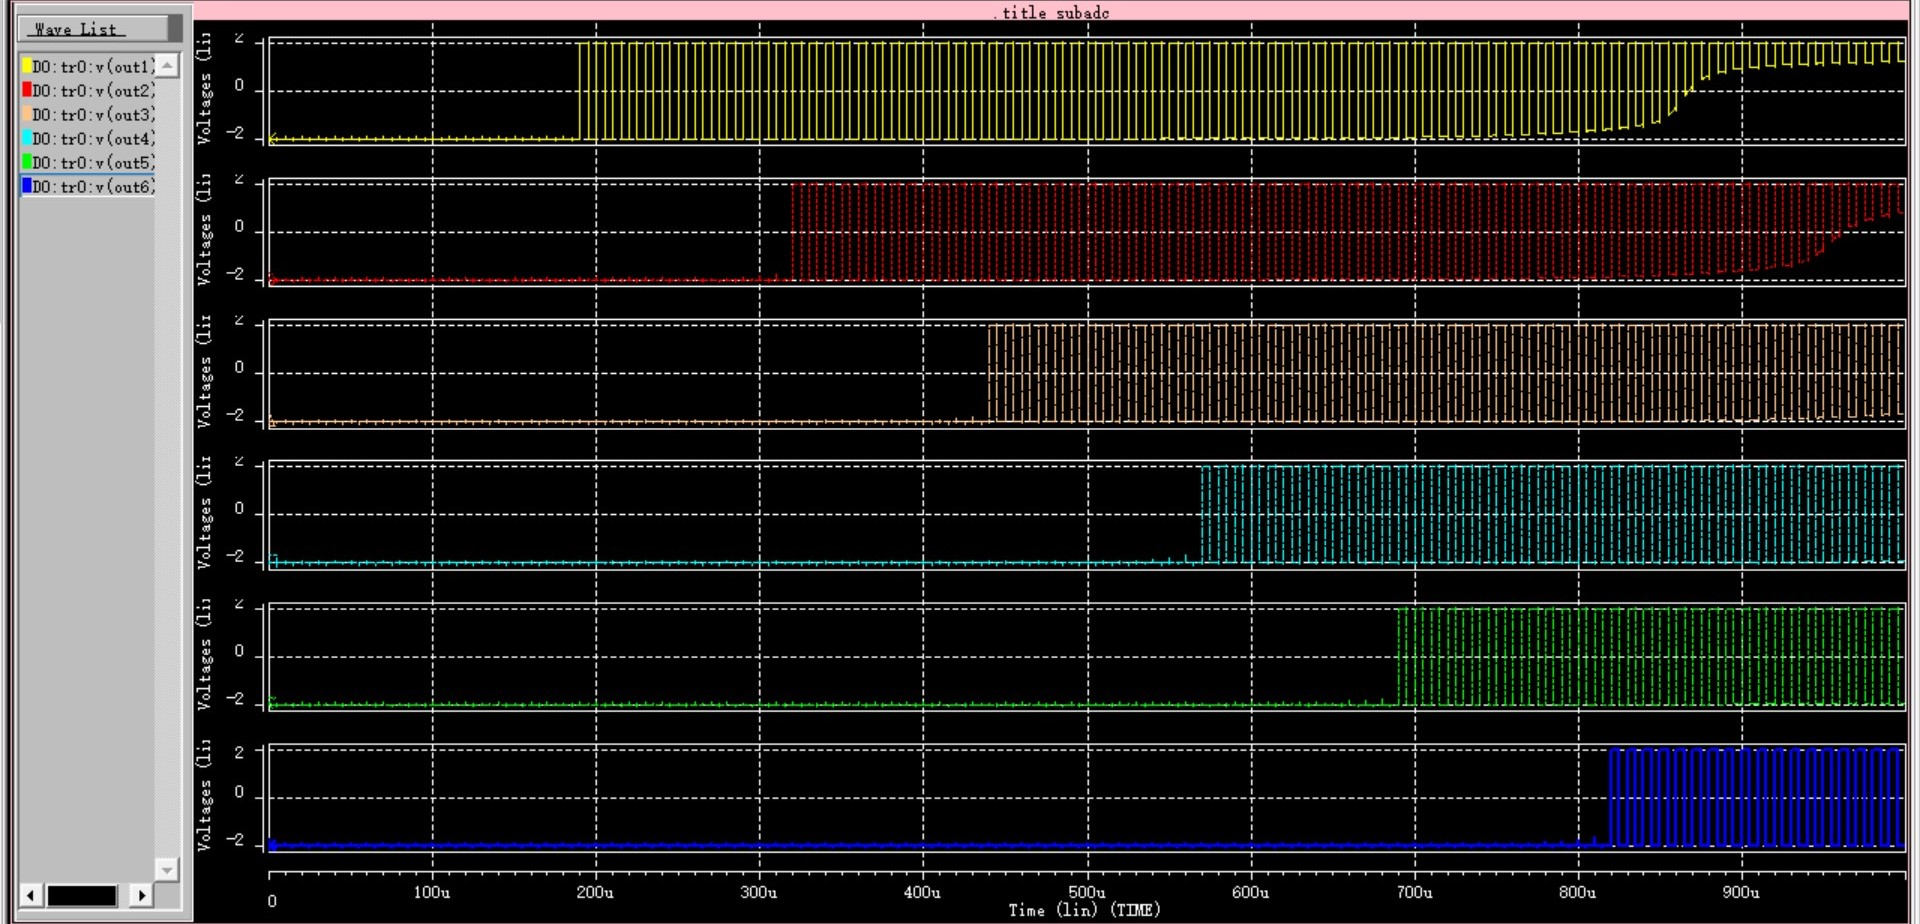
\includegraphics[width=10cm]{subADC_out}
			\caption{\label{fig:subADC_out}sub-ADC的六个输出}
		\end{figure}	
	\end{frame}

	\begin{frame}
		\ftitle{MDAC电路}
		利用电压加法电路,直接将各比较器输出电压缩放后相加,得到从0-6V的叠加信号,
		减去3V固定电平,使得输出信号在$[-3V,\ 3V]$范围内。在利用减法电路与放大的输入信号做差,
		就能够实现余量放大功能	
	\end{frame}


	\begin{frame}
		\ftitle{MDAC电路}
		\par MDAC电路原理图如\autoref{fig:MDAC_multisim}。
		\begin{figure}[H]
			\centering
			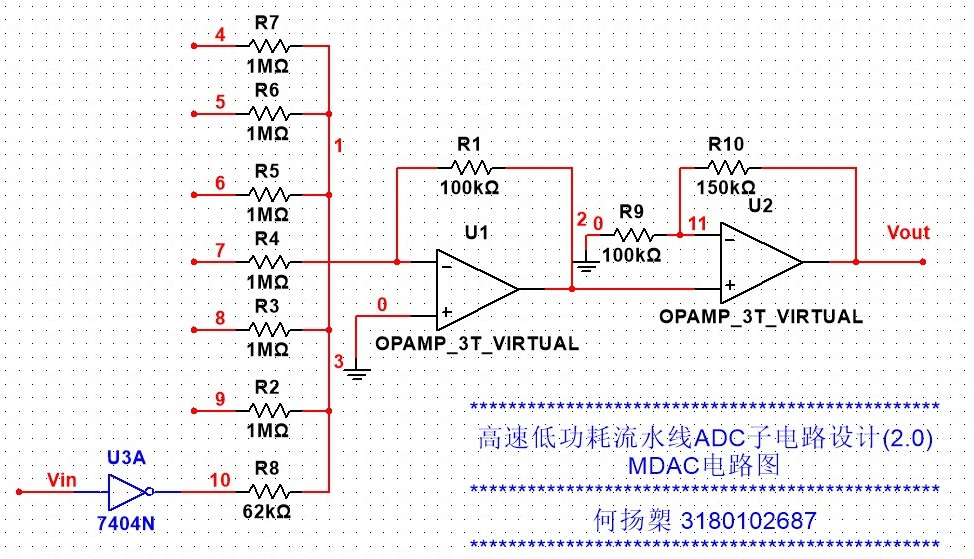
\includegraphics[width=9cm]{MDAC_multisim}
			\caption{\label{fig:MDAC_multisim}MDAC电路原理图}
		\end{figure}		
	\end{frame}

	\begin{frame}
		\ftitle{MDAC电路}
		得到较为理想的输出图像如\autoref{fig:MDAC_clk_ref}。
		\begin{figure}[H]
			\centering
			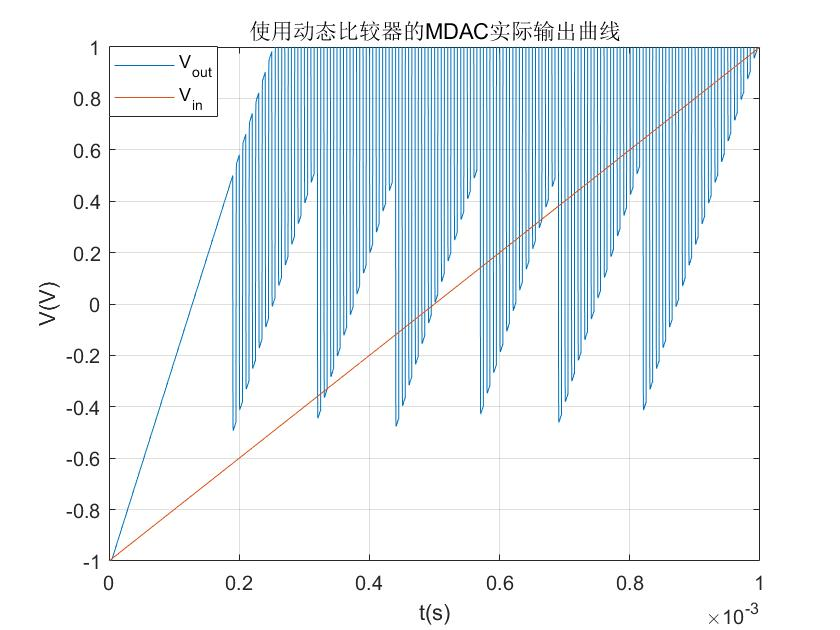
\includegraphics[width=8cm]{MDAC_clk_ref}
			\caption{\label{fig:MDAC_clk_ref}MDAC电路输出}
		\end{figure}	
	\end{frame}

	\begin{frame}
		\ftitle{第一级子电路}
		根据HSPICE仿真,第一级子电路总体参数如\autoref{tab:para}
		\begin{table}[H]
			\centering
			\caption{\label{tab:para}第一级子电路参数}
			\begin{tabular}{|c|c|}
				\hline
				工作电压 & $ \pm 2V $ \\ \hline
				最大工作速率 & $1MSPS$ \\ \hline
				比特数 & $2.5$  \\ \hline
				功耗 & $134.8mW$  \\ \hline
			\end{tabular}
		\end{table}
	\end{frame}

	\begin{frame}
		\ftitle{第一级子电路}
		\par 第一级子电路原理图如\autoref{fig:ALL_multisim}。
		\begin{figure}[H]
			\centering
			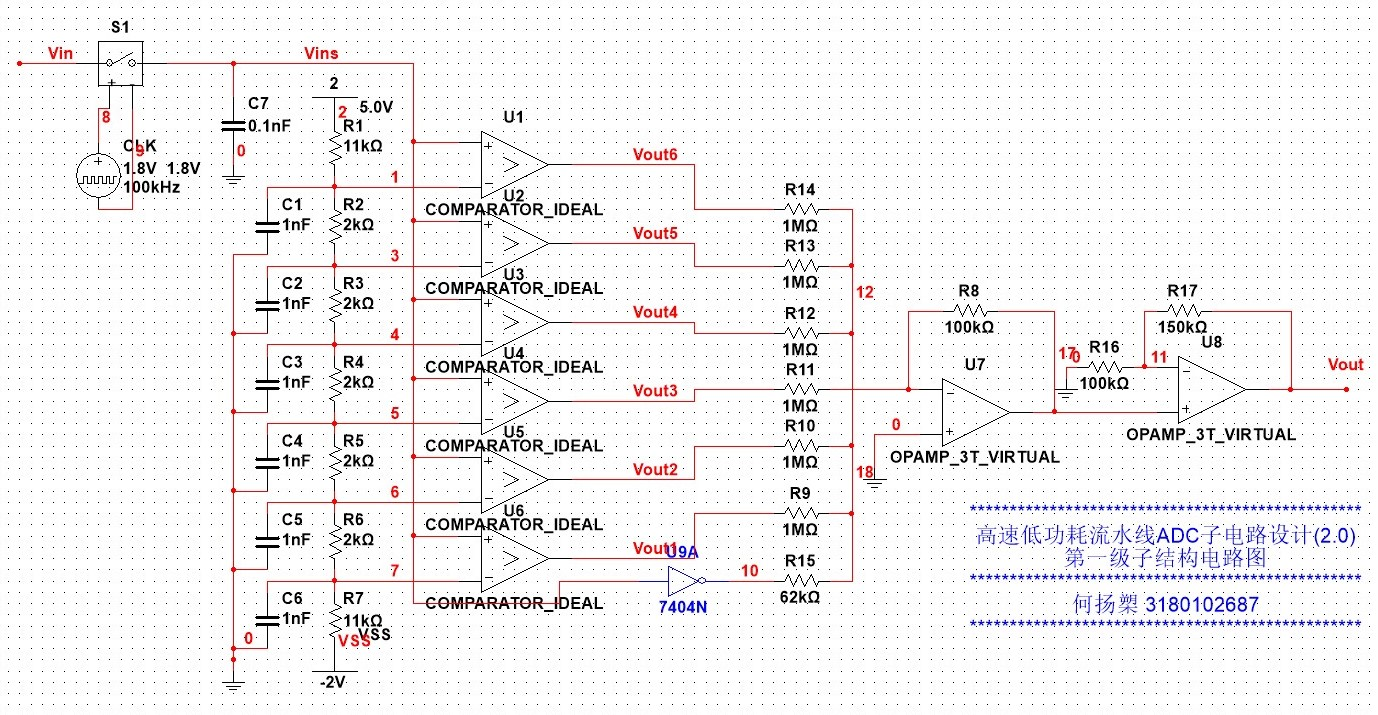
\includegraphics[width=9cm]{ALL_multisim}
			\caption{\label{fig:ALL_multisim}第一级子电路原理图}
		\end{figure}
	\end{frame}

	\begin{frame}
		\ftitle{第一级子电路}
		受限于运算放大器子结构的工作速率不能太高,否则,由于运算放大器响应速率低,
    	将导致MDAC中的加法电路无法正常工作,从而导致子结构整体输出错误。
		\begin{table}
        \centering
        \caption{\label{tab:SR_com}子结构中各模块压摆率对比}
        \begin{tabular}{|c|c|c|}
            \hline
            模块 & $SR(V/\mu s)$ \\ \hline
            栅压自举式开关 & $5074$ \\ \hline
            动态比较器 & $5.09\times 10^4$ \\ \hline
            运算放大器 & $10.72$ \\ \hline
            sub-ADC & $5.09\times 10^4$ \\ \hline
            MDAC & $10.72$ \\ \hline
        \end{tabular}
    	\end{table}
	\end{frame}

	\begin{frame}
		\ftitle{第一级子电路}
		\par 利用HSPICE仿真,可以得到第一级子电路在1MSPS工作速率下
		的总体功耗,如\autoref{fig:all_power}。
		\par 根据此第一级子电路估计,完整的流水线ADC电路功率约5个子结构加上数字
		校正电路的功耗之和,保守估计大约$ 1W $,由于电路无法工作以大于10MSPS的速率
		工作,因此无法得知约1GSPS速率下功耗。
		\begin{figure}[H]
			\centering
			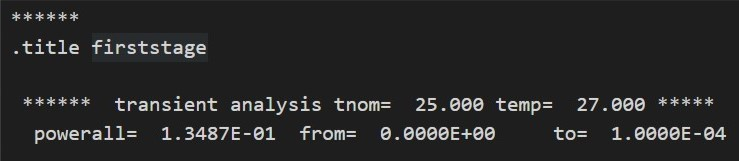
\includegraphics[width=8cm]{all_power}
			\caption{\label{fig:all_power}第一级子电路功率出(10MSPS)}
		\end{figure}
		\begin{align}
			P_{sub} = 134.8mW
		\end{align}
	\end{frame}

\section{References 参考文献}
\begin{frame}[allowframebreaks]
	\ftitle{Bibliography}
	中文内容显示
	The not so short introduction to LATEX2$\varepsilon$ \cite{Oetiker2015Latex} \\
	~\\
	The texbook \cite{knuth1984texbook}
    \label{Reference}
    \bibliographystyle{apalike}	   % different styles, such as ieee
    \bibliography{mybibliography}  % make reference list
\end{frame}

\section{Thanks 致谢}
\begin{frame}
	\ftitle{End}
	感谢!
\end{frame}


\end{document}
